\section{Methodology}

Parsplice is an HPC application with distinct workload phases and a well-known keyspace (Figure~\ref{fig:keyspace-size}).
\begin{figure*}[tbh]
  \noindent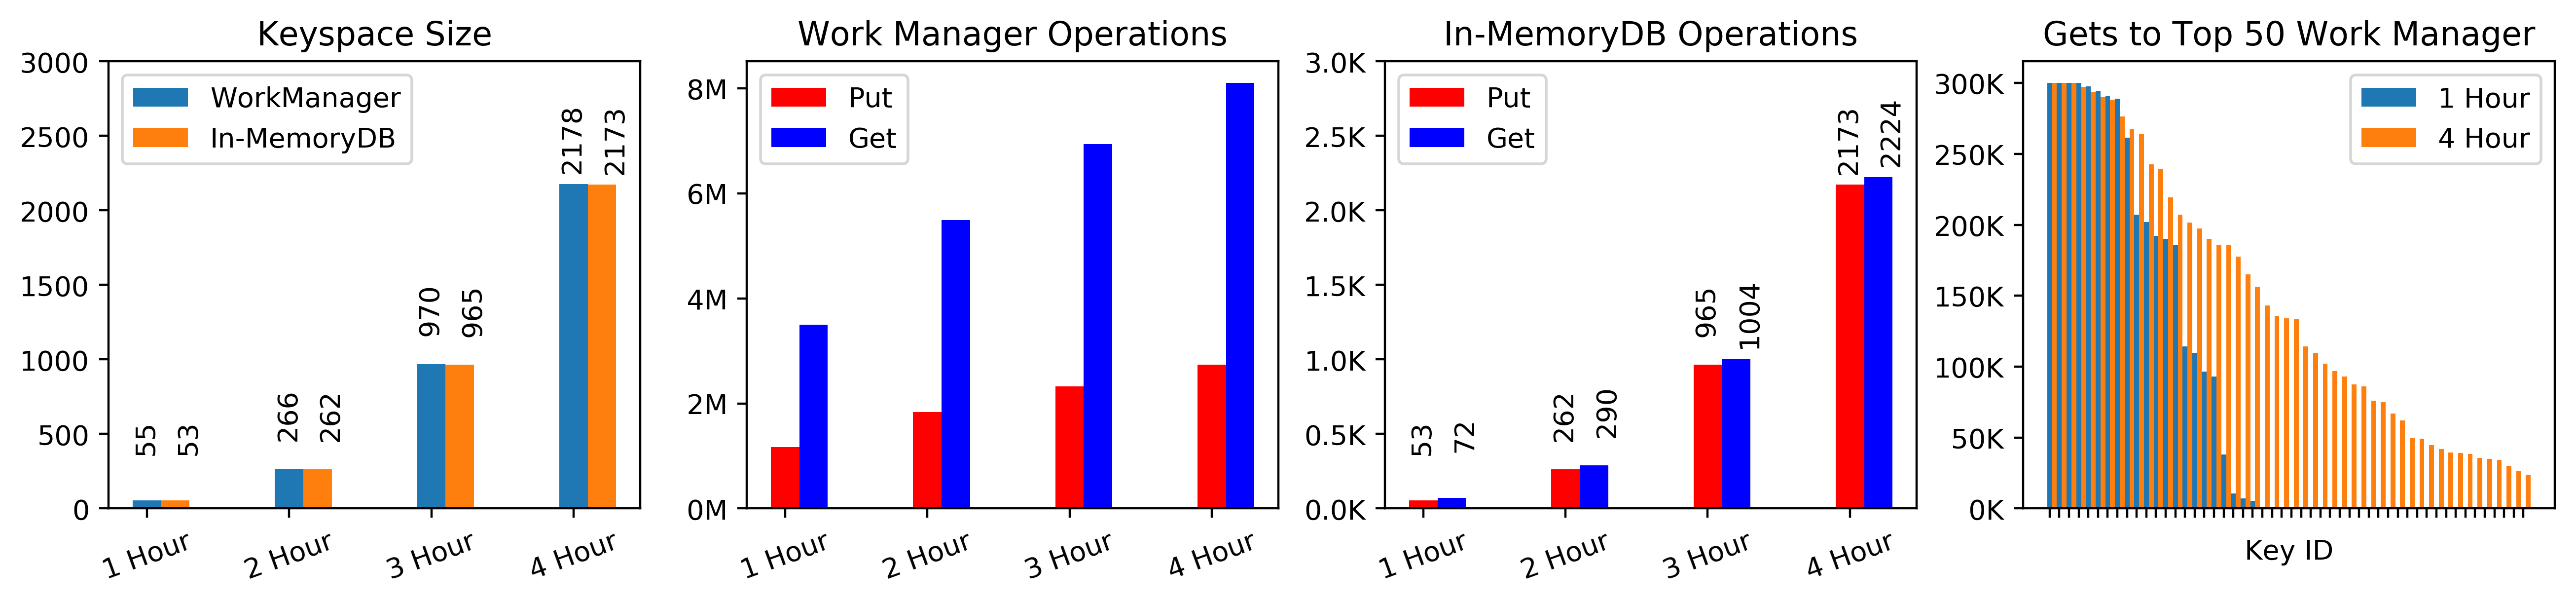
\includegraphics[width=1\textwidth]{figures/keyspace-size.png}\\
  \caption{The keypspace grows in a structured way, so we can predict the
  number and popularity of hot keys 
  \label{fig:keyspace-size}}
\end{figure*}

\begin{figure*}[tbh]
  \noindent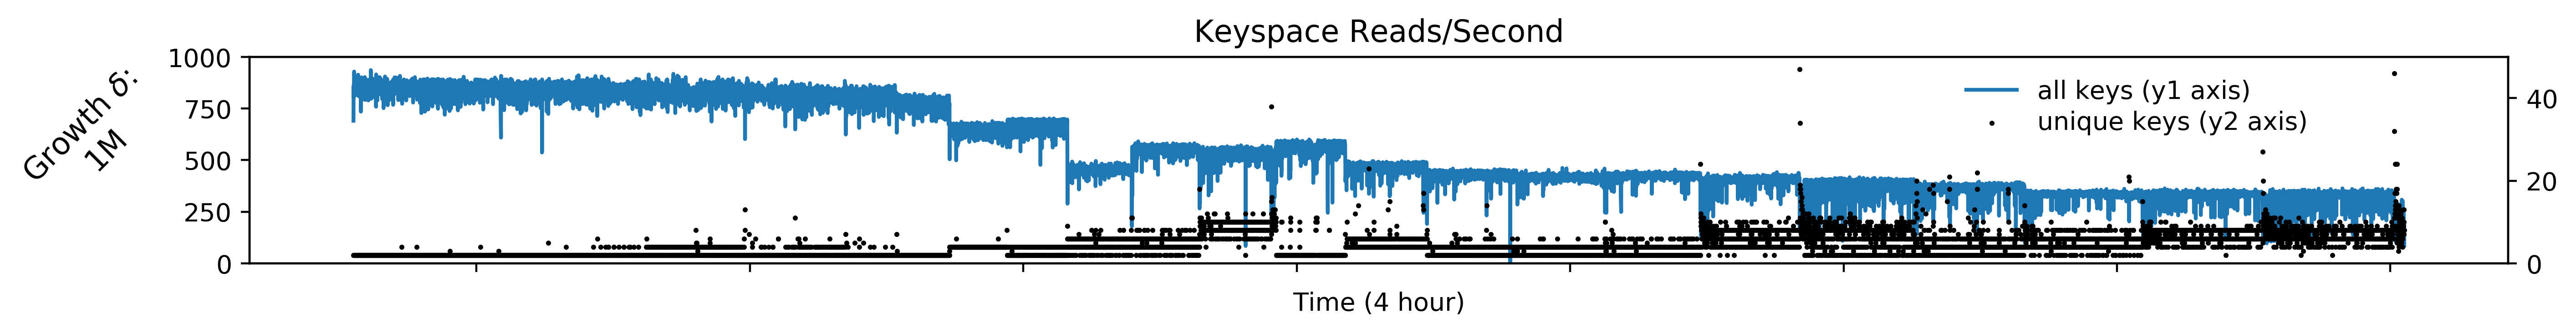
\includegraphics[width=1\textwidth]{figures/keyspace-regimes-4hr.png}\\
  \caption{Access patterns for a growth \(\delta\) of 1M shows similiar
  behavior to 100K but on different time scales.
  \label{fig:keyspace-regimes-4hr}}
\end{figure*}

Part 1: Parsplice architecture uses a backend KV store
\begin{itemize}
  \item Single Node DB (LevelDB, BerkeleyDB) is insufficient
  \item Distributed KV store solves sync problem and enables load balancing
  \item HXHIM 
\end{itemize}

Part 2: As Parsplice simulates, entropy increases resulting in keyspace
inbalance (Figure~\ref{fig:keyspace-regimes} shows how imbalance controlled by
``growth rate")
\begin{itemize}
  \item Mantle (approach/API) to explore dynamic load balancing policies
  \begin{itemize}
    \item quantifies effect of load balancing
    \item formalized effective FS balancers
    \item debugging tool 
  \end{itemize}
  \item HXHIM is a good fit because it has migration mechanisms for load balancing
  \begin{itemize}
    \item bulk operations (\texttt{put/get()})
    \item key partitioners
    \item secondary indices
  \end{itemize}
  \item we need a way to learn these regimes
  \begin{itemize}
    \item Figure~\ref{keyspace-regimes-4hr} shows the same phases as 100K but that the timestamps affected by delay
  \end{itemize}
\end{itemize}

Results should show, In order from most likely to least likely:

\begin{enumerate}

  \item HPC key-value store workloads are structured (because they are mostly
  workflows and simulations) that their job phases can be learned and exploited
  using dynamic load balancing policies.

  \item HPC key-value store workloads are so structured that one
  policy-fits-all

  \item HPC key-value store workloads are not structured enough to be learned

  \item HPC key-value store workload hotspots/flash crowds are too fast to be
  exploited

\end{enumerate}



%\begin{itemize}
%  \item C bindings for Mantle
%\end{itemize}
%
%\subsection{Pluggable Interfaces}
%
%\begin{figure}[tb]
%  \noindent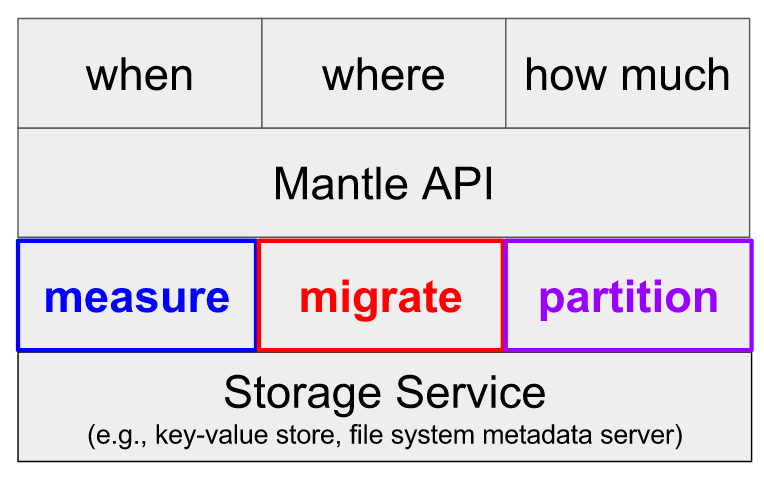
\includegraphics[width=19pc,angle=0]{figures/mantle-pluggable-interfaces.png}\\
%  \caption{The storage service must: \textcolor{blue}{\textbf{measure}}
%  resource usage, \textcolor{red}{\textbf{migrate}} resources, and
%  \textcolor{purple}{\textbf{partition}} resources. }
%  \label{fig:mantle-pluggable-interfaces}
%\end{figure}
%
%\subsubsection{Measure}
%
%The metrics measured should help the system decide ``when" to migrate server
%load. They should:
%
%\begin{itemize}
%  \item tell us about the state of the server or cluster
%  \item provide some value of load, so we can partition/send it
%\end{itemize}
%
%In Ceph: global and local metrics ({\it e.g.}, CPU utilization, file system operation counts) \\
%
%In HXHIM: ???\\
%
%\subsubsection{Migrate}
%
%In Ceph: \texttt{export\_dir()}
%
%In HXHIM: \texttt{mdhimBPut()}, \texttt{mdhimBGet()}, ``adjusting ... keys" ???
%
%\subsubsection{Partition}
%
%In Ceph: subtrees and directory fragments
%
%In HXHIM: secondary indices, cursor types, bul operations
